The \textit{Notification} module is currently used for sending notifications to
the user upon account creation or when the user tries to recover a lost account.
The module can however be expanded in future to allow other notification 
services and hence the decision to include this as a major module in the system
and not as a submodule of the User Management module.

\subsection{Scope}
The scope for the Notification modules is shown in Figure \ref{fig:notificationScope}.
\begin{figure}[H]
	\begin{center}
		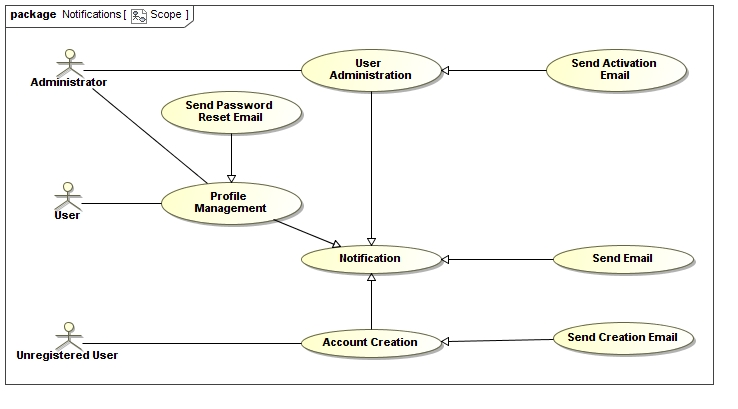
\includegraphics[scale=0.38]{../Diagrams and Charts/Notifications/Scope.jpg}
		\caption{Notification Scope}
		\label{fig:notificationScope}
	\end{center}	
\end{figure}

These use cases will be used by the User Management Module to assist with the
user authentication and recovering of lost accounts. The module however provides
general functionality to send emails which can be used by any other module that
may require this in future.

\subsection{Send Activation Email}
The \textit{Send Activation Email} use case is concerned with with sending
a new created managed user an email on how to setup there password. Important to
note is that the user's account has been activated as it was created by an
administrator, however the administrator should not have control off selecting a
password for the user as this will violate general security principles.

\subsubsection{Service Contract}
The service contract for sending an activation email upon account creation is 
shown in Figure \ref{fig:sendActivationEmailServiceContract}

\begin{figure}[H]
	\begin{center}
		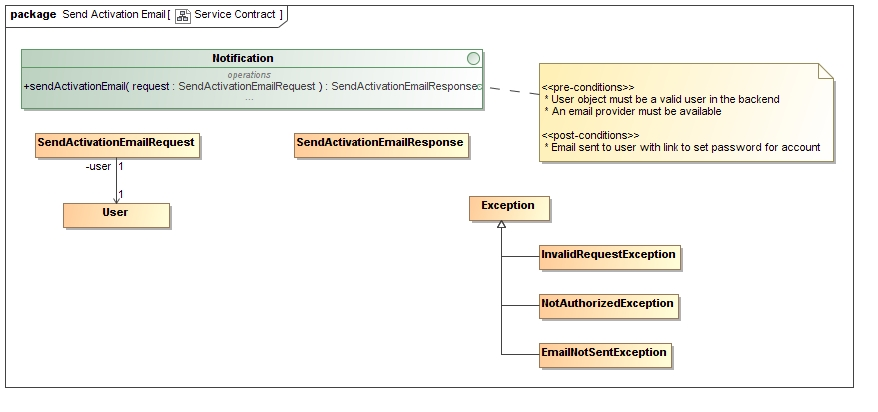
\includegraphics[scale=0.38]{../Diagrams and Charts/Notifications/Send Activation Email Service Contract.jpg}
		\caption{Send Activation Email Service Contract}
		\label{fig:sendActivationEmailServiceContract}
	\end{center}	
\end{figure}

\subsubsection{Functional Requirements}
The lower level services required by the send activation email service to either
check the pre-conditions or address the post-conditions is shown 
Figure \ref{fig:sendActivationEmailFunctionalRequirements}.
\begin{figure}[H]
	\begin{center}
		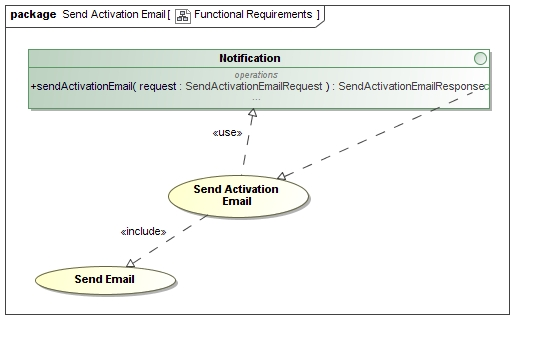
\includegraphics[scale=0.38]{../Diagrams and Charts/Notifications/Send Activation Email Functional Requirements.jpg}
		\caption{Send Activation Email Functional requirements}
		\label{fig:sendActivationEmailFunctionalRequirements}
	\end{center}	
\end{figure}



\subsection{Send Creation Email}
The \textit{Send Creation Email} use case is concerned with with sending
a new unmanaged user an email on how to activate their account.

\subsubsection{Service Contract}
The service contract for send a creation email is shown in 
Figure \ref{fig:registerNodeHeartbeatServiceContract}.
\begin{figure}[H]
	\begin{center}
		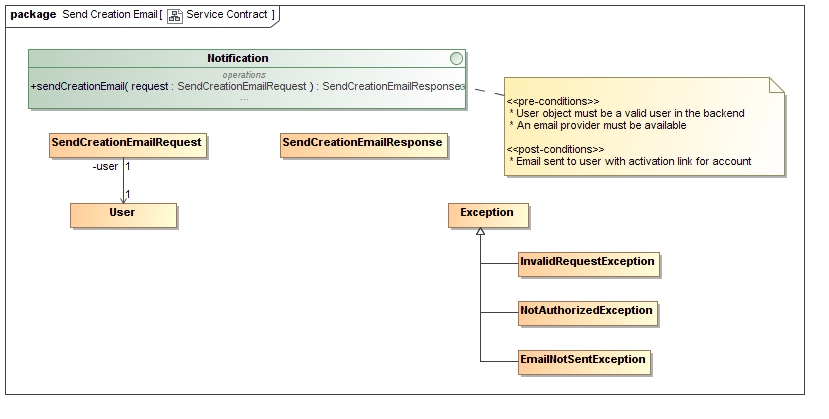
\includegraphics[scale=0.38]{../Diagrams and Charts/Notifications/Send Creation Email Service Contract.jpg}
		\caption{Send Creation Email Service Contract}
		\label{fig:sendCreationEmailServiceContract}
	\end{center}
\end{figure}

\subsubsection{Functional Requirements}
The lower level services required by the send creation email service to either
check the pre-conditions or address the post-conditions is shown 
Figure \ref{fig:sendCreationEmailFunctionalRequirements}.
\begin{figure}[H]
	\begin{center}
		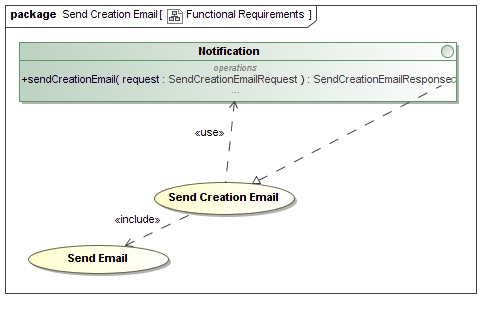
\includegraphics[scale=0.38]{../Diagrams and Charts/Notifications/Send Creation Email Functional Requirements.jpg}
		\caption{Send Creation Email Functional Requirements}
	  \label{fig:sendCreationEmailFunctionalRequirements}
	\end{center}
\end{figure}



\subsection{Send Email}
The \textit{Send Email} use case is concerned with with sending a body of
content to a specified receipt. The use case can be used as is, but it is
advised to rather make use of one of the wrapper use cases.

\subsubsection{Service Contract}
The service contract for sending an email is shown in 
Figure \ref{fig:registerNodeHeartbeatServiceContract}.
\begin{figure}[H]
	\begin{center}
		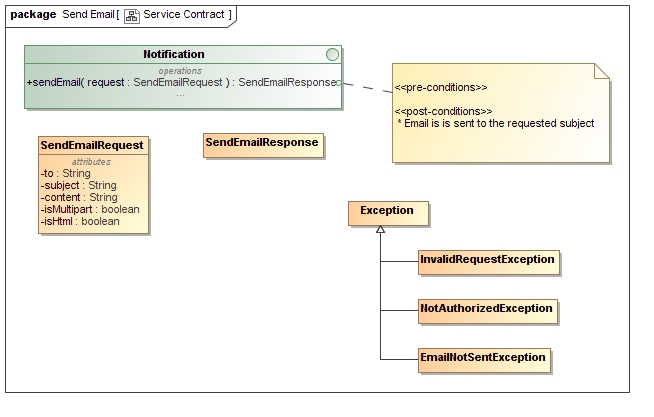
\includegraphics[scale=0.38]{../Diagrams and Charts/Notifications/Send Email Service Contract.jpg}
		\caption{Send Email Service Contract}
		\label{fig:sendEmailServiceContract}
	\end{center}	
\end{figure}

\subsubsection{Functional Requirements}
The lower level services required by the send email service to either
check the pre-conditions or address the post-conditions is shown 
Figure \ref{fig:sendEmailFunctionalRequirements}.
\begin{figure}[H]
	\begin{center}
		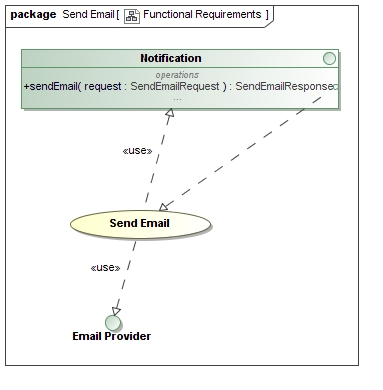
\includegraphics[scale=0.38]{../Diagrams and Charts/Notifications/Send Email Functional Requirements.jpg}
		\caption{Send Email Functional Requirements}
		\label{fig:sendEmailFunctionalRequirements}
	\end{center}	
\end{figure}



\subsection{Send Password Reset Email}
The \textit{Send Password Reset Email} use case is concerned with with sending
a user instructions on how to go about to reset there lost account password.

\subsubsection{Service Contract}
The service contract for sending a password reset email is shown in 
Figure \ref{fig:registerNodeHeartbeatServiceContract}.
\begin{figure}[H]
	\begin{center}
		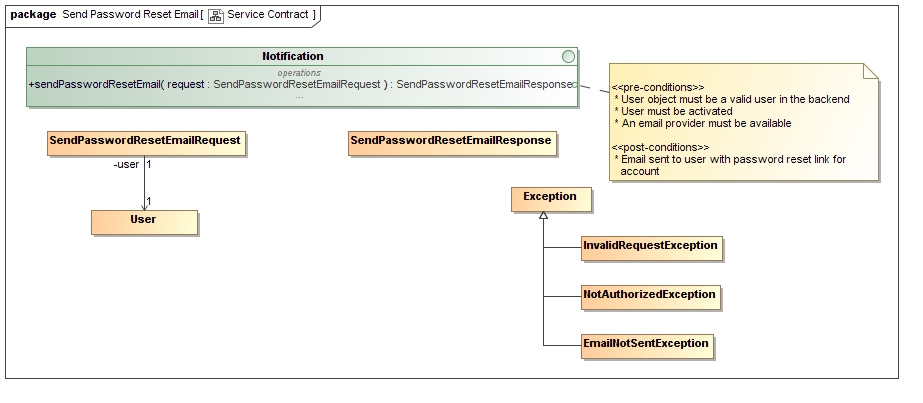
\includegraphics[scale=0.38]{../Diagrams and Charts/Notifications/Send Password Reset Email Service Contract.jpg}
		\caption{Send Password Reset Email Service Contract}
		\label{fig:sendPasswordResetMailServiceContract}
	\end{center}
\end{figure}

\subsubsection{Functional Requirements}
The lower level services required by the send password reset email service to 
either check the pre-conditions or address the post-conditions is shown 
Figure \ref{fig:sendPasswordMailFunctionalRequirements}.
\begin{figure}[H]
	\begin{center}
		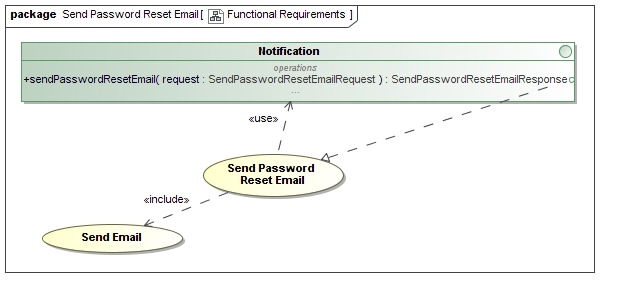
\includegraphics[scale=0.38]{../Diagrams and Charts/Notifications/Send Password Reset Email Functional Requirements.jpg}
		\caption{Send Password Reset Email Functional Requirements}
	  \label{fig:sendPasswordMailFunctionalRequirements}
	\end{center}
\end{figure}


